% context: 9th-grade physics classwork, in-class review the day before the 1.7 quiz
% topic: significant figures, rounding, scientific notation, reading a ruler,
%        unit conversion, average speed
% structure: two pages, problems widely spaced; every question asks for one unit
% convention: long decimals are typeset with \num{} (siunitx), which groups the
%        digits in threes with a thin space: \num{0.000000532} -> 0.000 000 532
\documentclass[12pt, twoside]{article}
%\documentclass[12pt, twoside]{article}
\usepackage[letterpaper, margin=1in, headsep=0.2in]{geometry}
\setlength{\headheight}{0.6in}
%\usepackage[english]{babel}
\usepackage[utf8]{inputenc}
\usepackage{microtype}
\usepackage{amsmath}
\usepackage{amssymb}
%\usepackage{amsfonts}
\usepackage[nomessages]{fp} %\FPeval{\var-name}{2*sin(pi/6)}
\usepackage{siunitx} %units in math. eg 20\milli\meter
\usepackage{yhmath} % for arcs, overparenth command
\usepackage{tikz} %graphics
\usetikzlibrary{quotes, angles, arrows, arrows.meta}
\usepackage{graphicx} %consider setting \graphicspath{{images/}}
\usepackage{parskip} %no paragraph indent
\usepackage{enumitem}
\usepackage{multicol}
\usepackage{venndiagram}

\usepackage{fancyhdr}
\pagestyle{fancy}
\fancyhf{}
\renewcommand{\headrulewidth}{0pt} % disable the underline of the header
\raggedbottom
\hfuzz=2mm %suppresses overfull box warnings

\usepackage{hyperref}
\usepackage{float}

\title{Physics}
\author{Chris Huson}
\date{October 2026}

\fancyhead[LE]{\thepage}
\fancyhead[RO]{\thepage \\ Nickname: \hspace{2.25cm} \,\\ \,}
\fancyhead[LO]{La Scuola d'Italia / Huson / Physics \\* 1 October 2026}

\begin{document}

\subsubsection*{1.6 Classwork: Measurement review}

\textbf{Reference (provided).} \quad
average speed $= \dfrac{\text{distance}}{\text{time}}$ \\[0.1cm]
1 m $\approx$ 3.28 ft \quad 1 km = 1000 m \quad 1 m = 100 cm \quad 1 cm = 10 mm \\
1 h = 3600 s \quad 1 yr $\approx$ 365.25 days \quad 1 week = 7 days

\vspace{0.3cm}

\begin{enumerate}[itemsep=0.6cm]

\item Write down the number of significant digits in each measurement.
  \begin{multicols}{3}
    \begin{enumerate}[itemsep=0.5cm]
      \item 3.08 m
      \item 0.0062 kg
      \item 40.0 s
      \item 1.200 m
      \item \num{0.0005010} m
      \item $2.998 \times 10^{8}$ m/s
    \end{enumerate}
  \end{multicols}

\item Round each value to three significant figures. Copy the calculator display
  followed by three dots, then round: $\sqrt{2} = 1.4142135\ldots \approx 1.41$
  \begin{multicols}{2}
    \raggedright
    \begin{enumerate}
      \item $\sqrt{11}$
      \item One mile, 1609.344 m
    \end{enumerate}
  \end{multicols} \vspace{1.0cm}

\item Write in scientific notation, rounded to three significant figures.
  \begin{multicols}{2}
    \raggedright
    \begin{enumerate}
      \item The diameter of the Sun, 1{,}392{,}700~km
      \item The time light takes to cross a meter stick, \num{0.00000000333564} s
    \end{enumerate}
  \end{multicols} \vspace{1.6cm}

\item Write each value as an ordinary decimal number.
  \begin{multicols}{2}
    \raggedright
    \begin{enumerate}
      \item The diameter of a red blood cell, $7.8 \times 10^{-6}$ m
      \item The distance from the Earth to the Sun, $1.496 \times 10^{8}$ km
    \end{enumerate}
  \end{multicols} \vspace{1.4cm}

\item Usain Bolt ran 100 m in 9.58 s. What was his average speed in kilometers per
  hour?

\newpage

\item The bar below is measured with a centimeter ruler marked in millimeters.

\begin{center}
\begin{tikzpicture}[scale=1.05]
  \draw[fill=gray!20] (0,0.18) rectangle (5.83,0.78);
  \draw[thick] (-0.5,0) -- (10.6,0);
  \foreach \x in {0.1,0.2,...,9.95}{\draw (\x,0) -- (\x,-0.14);}
  \foreach \x in {0,1,2,3,4,5,6,7,8,9,10}{\draw[thick] (\x,0) -- (\x,-0.3) node[below] {\small \x};}
  \node[right] at (10.7,-0.15) {\small cm};
\end{tikzpicture}
\end{center}

  \begin{enumerate}[itemsep=1.0cm]
    \item Record the length of the bar. Include one estimated digit --- the last
      digit, the one you are not certain of.
    \item How many significant figures does your measurement have?
    \item Write your measurement in meters.
  \end{enumerate} \vspace{1.0cm}

\item Convert between units, rounding to three significant figures. Write each
  conversion as a single chain of fractions and show the units cancelling.
  \begin{enumerate}[itemsep=2.6cm]
    \item The Burj Khalifa is 828 meters tall. What is its height in feet?
    \item The elevators in the Shanghai Tower climb at 20.5 meters per second. What
      is this speed in kilometers per hour?
  \end{enumerate} \vspace{2.4cm}

\item Fingernails grow about 3.5 centimeters per year. How many millimeters does a
  fingernail grow in one week?

\end{enumerate}
\end{document}
